\chapter{Critical Success Factor Analysis Based on Feaure Selection}
\label{ch:2_csf_fs}

\begin{quotation}[]{Paulo Freire}
No one knows it all. No one is ignorant of everything. We all know something. We are all ignorant of something.
\end{quotation}

Critical Success Factor (CSF) is a management term for an element that is necessary for an organization or project to achieve its mission. CSFs represent the principal assets or areas that must be given investments to achieve better results. CSF analysis is one challenger strategic management tool, wich can provide a robust and very practical assessment for strategic planners.

The identification of the most significative information for one problem is referred to as feature selection by the signal processing and data mining areas, as well as it can be formulated as a principal component problem, which is a widely adopted signal processing technique for data visualization and feature extraction. Feature selection aims to select a subset of relevant information from a larger dataset, in order to improve: data visualization and data understanding, storage requirements, dimensionality, processing time, discriminative sensing, and to overcome overfitting problems to improve prediction and classification performance \cite{chandrashekar2014survey}.

Recursive Feature Elimination (RFE) is a feature selection method for small sample classification problems. RFE seeks to improve generalization performance by recursivelly removing the least significant features whose deletion will have the least effect on training errors, according to the higher variance measured from the features \cite{chen2007enhanced}.

We propose a critical factors analysis based on Principal Compoment Analytis (PCA) for visual discriminant analysis and based on RFE combined with Support Vector Machine (SVM) \cite{hearst1998support}, applied to the survey that evaluates the IT governance of brazilian public organizations, in order to identify the CSF for IT governance of the public sector according to TCU. Results show how PCA can make the data discriminative and that SVM is the classifier that best performs and obtains an accuracy of 91.42\% to learn and classify according to TCU's IT governance evaluation of brazilian public sector. Finally, SVM is used to highlight the more significant features identified by RFE, wich are limilar to CSFs previsously identified by a qualitative analysis of the same datased.

This chapter is organized as follows. In Section \ref{sec:relatedworks}, related works are discussed. Section \ref{sec:datamodel} presents the data model and the evaluated datasets. Section \ref{sec:csf_fs} describes the proposed approach for critical success factors analysis. Section \ref{sec:experimentalresults} discusses the experimental validation and presents the results, and Section \ref{sec:conclusion} draws the conclusions.

\section{Related Works}
\label{sec:relatedworks}

Fink and Sukenik \cite{fink2011effect} explore the relationships among IT infrastructure capability and IT business value using PCA applied to all indicators of their study, resulting into 11 factors, with the first factor accounting for only 27.9\% of the variance. This technique was used because the PCA extracts orthogonal factors that overcome the problem of multicollinearity.

Ramos \emph{et al} \cite{ramos2016information} propose an overview regarding the evolution of scientific research on IT Governance critical success factors within the domain of public administration. By means of bibliometric analysis it was investigated seminal works regarding this theme, considering the characteristic key words found during our analysis. The results present 64 critical success factors with high impact on IT governance.

Guyon \emph{et al} \cite{guyon2002gene} propose a method of gene selection utilizing Support Vector Machine methods based on Recursive Feature Elimination (RFE) and demonstrate that the selected genes yield better classification performance and are biologically relevant to cancer.  The proposed method eliminates gene redundancy automatically and yields better and more compact gene subsets. 

To the best of our knowledge, we are the first to propose a critical factors analysis based on PCA for visual discriminant analysis and based on RFE combined with SVM for CSF identification from IT governance data.

\section{Data Model}
\label{sec:datamodel}

The brazilian Federal Court of Accounts (TCU, in Portuguese) surveys data regarding IT practices of brazilian public organizations in order to audit IT governance. The dataset with a consolidate view about the answers for this surgey the IT governance index is called iGovTI. The iGovTI is composed by 201 multiple choice questions, used for ranking according to their IT governance, submmited to 349 organizations. The TCU computes the IT governance index and classifies the IT governace of each organization. Additionally, Ramos \emph{et al} \cite{ramos2016information} classifies each question regarding its relevance for IT governance through a qualitative analysis, and identify the CSFs for selected IT managers regarding IT governance.

\section{An approach for Critical Success Factors Analysis}
\label{sec:csf_fs}

In this section we propose an approach for Critical Success Factors Analysis based on visual discriminant analysis and based on feature selection, in orde to identify the CSFs for IT governance according to iGovTI. Initially we conduct an analysis based on PCA to evaluate the relevante of each feature according to their variance, and use the 2 most relevant features for a visualization of the iGovTI ranking. Furthermore, we propose a critical success factors analysis based on SVM for classification and based on RFE for identification of the most relevant factors.

\subsection{Visual Discriminant Analysis based on PCA}

PCA is a statistical technique commonly used for dimensionality reduction. It uses an orthogonal transformation to convert a set of correlated variables into a set of linearly uncorrelated variables, where the first principal components have the largest variance.

PCA is also used for finding patterns in data of high dimension and for highlighting its discrinative characteristics and strucutres, throught an orthogonal basis transformation into new basis, by diagonalizing the centered covariance matrix of a data set {Xk E RNlk = 1, ... ,f}, defined by C = ((Xi - (Xk))(Xi - (Xk))T). The coordinates in the Eigenvector basis are called principal components. The size of an Eigenvalue >. corresponding to an Eigenvector v of C equals the amount of variance in the direction of v. PCA is usually used for signal denoising, blind source separation, data compression, data visualization, feature extraction and dimensionality reduction, where a reduced number of features is extrated retaining as much information as possible \cite{jolliffe1986principal}.

PCA combines similar (correlated) attributes and creates new ones. Superior to original attributes. 

Feature selection doesn't combine attributes. Just evaluates their quality, predictive power and select the best set. 

Benefit in PCA is that combination of N attributes is better than any individual attribute. Disadvantage is in harder explanation what exactly that PCA component means.

describe PCA matematically here? acho que talvez seja melhor fazer uma descricao mais alto nível e voltar depois se sobrar tempo

descrever cmo os dados são aplicados ao pca e apresentar os resultados obtidos

A Figura 1 mostra geometricamente a ACP de duas variáveis X1 e X2. A nuvem de pontos representa o diagrama de espalhamento destas duas variáveis. Conforme explicado, o primeiro passo é o cálculo da matriz de variância-covariância e em seguida se aplica a EVD. Verifica-se que a CP1, denominado CP principal (com a maior variância), é ortogonal à segunda CP (CP2 com a menor variância). Note que as duas variáveis são perpendiculares porque as variáveis obtidas pela ACP são independentes. Logo, após a aplicação da ACP, ao invés de representar os dados por meio de duas variáveis correlacionadas X1 e X2, eles podem ser representados por duas variáveis independentes Y1 e Y2. Dada a elevada correlação entre X1 e X2, verifica-se que as duas variáveis X1 e X2 podem ser aproximadas por uma única variável Y1 na Figura 1.

Figura 1 – Representação e Rotação do Componente Principal
Fonte: Desenvolvido pelos autores

A Figura 1 reforça a ideia da ACP cujo objetivo inicial é a identificação de planos e linhas que representem um conjunto de pontos em um espaço com um número menor de variáveis tendo em vista as possíveis correlações que podem existir entre as variáveis originais.
Assim, para o método da estatística multivariada ACP utilizar todas variáveis, separa-se a informação útil da informação redundante (Finkler, 2003). Ressalta-se que a ACP é um dos primeiros passos para outras análises multivariadas, sendo um dos métodos mais comuns empregados na análise de informações (Sabin, Ferrão e Furtado, 2004; Silva et al.,2012).

\subsection{iGovTI classification}

SVM é um método supervisionado de aprendizagem de máquina, não probabilístico, baseado na teoria de aprendizagem estatística, usado para classificação, regressão e detecção de padrões. MVS pode ser aplicado por meio de dois passos: o primeiro passo é o treinamento de um modelo a partir de um determinado conjunto de dados; o segundo consiste em estimar a classificação de dados a partir da aplicação do modelo treinado. 
Quando aplicado para classificação, MVS busca a identificação de um hiperplano que separa os dados em classes distintas, por meio de uma margem máxima entre duas classes de dados. Desta forma, um conjunto de dados é linearmente separável se for possível dividir seus dados em duas classes, por meio um hiperplano, conforme na figura a seguir. 

Figura 2 – Separação Linear por Margem Máxima

Dado um conjunto de dados previamente classificados, (xi, yi), xi ∈ Rn, yi ∈ {1, −1}, i = 1, . . . , l, um classificador linear pode ser definido por: wT ⋅ x + b = 0, desta forma o hiperplano ótimo é definido pelos valores ótimos do vetor de pesos wi e do bias bi, de forma que wT ⋅ x + b = 1 e wT ⋅ x + b = -1 representam respectivamente os vetores de suporte positivos e negativos, que são os pontos próximos à margem do hiperplano ideal. A margem máxima, entre os vetores de suporte, é definida por:

As funções de kernel têm o objetivo de projetar os vetores de variáveis de um conjunto de dados em um espaço de maior dimensão, para a classificação de classes originalmente apresentadas em espaços não separáveis linearmente. Com o aumento da dimensão, aumenta a probabilidade desses dados poderem ser linearmente separáveis. 
% Uma função kernel K(xi, xj) = φ(xi) T φ(xj) pode ser usada para treinar a MVS. Uma MVS linear tem φ(x) = x, assim uma função kernel linear pode ser representada por K(xi, xj) = xTi xj.
Foi adotada a estratégia "um contra um" (Knerr, Personnaz e Dreyfus, 1990), para a utilização de MVS para a classificação de muitas classes. Esta estratégia consiste em construir uma máquina vetor de suporte para cada par de classes. Para um problema com c classes, c(c-1)/2 MVSs são treinados para classificar as classes entre as c classes possíveis.

\subsection{CSF analysis based on SVM-RFE}

Dado um algoritmo de classificação, que possa estimar pesos para as variáveis de um conjunto de dados, o objetivo da Eliminação Recursiva de Variáveis (ERV), do inglês Recursive Feature Elimination (RFE) (Guyon, 2002), é selecionar variáveis por meio da redução recursiva da quantidade de variáveis, eliminando recursivamente as variáveis de menor peso para classificação por meio do algoritmo adotado. 
Primeiramente, um modelo é treinado, utilizando o conjunto de dados inicial e o algoritmo selecionado, durante o treinamento são atribuídos pesos para cada variável, representando a importância de cada variável para a classificação. Em seguida, as variáveis com menor peso são eliminadas do conjunto de dados. Este processo, de treinamento, ordenamento de variáveis e eliminação de variáveis menos importantes, é repetido recursivamente até a obtenção do número desejado de variáveis, ou até a satisfação de alguma condição, como um limiar de taxa de erro de um algoritmo de classificação.
As variáveis com maiores pesos apresentam maior influência na classificação (Guyon, 2002). Desta forma, se um algoritmo de classificação apresenta boa acurácia, as variáveis com maiores pesos representam as variáveis que apresentam maior influência para a classificação.
MVS-ERV (Guyon, 2002) é uma aplicação da ERV utilizando os pesos obtidos por meio do treinamento utilizando MVS como algoritmo de classificação, para identificar as variáveis mais importantes para predições de classificação e eliminar recursivamente as variáveis que menos influenciam na classificação.

Recursive feature elimination is based on the idea to repeatedly construct a model (for example an SVM or a regression model) and choose either the best or worst performing feature (for example based on coefficients), setting the feature aside and then repeating the process with the rest of the features. This process is applied until all features in the dataset are exhausted. Features are then ranked according to when they were eliminated. As such, it is a greedy optimization for finding the best performing subset of features.

The stability of RFE depends heavily on the type of model that is used for feature ranking at each iteration. Just as non-regularized regression can be unstable, so can RFE when utilizing it, while using ridge regression can provide more stable results.

%Given an external estimator that assigns weights to features e.g., the coefficients of a linear model, recursive feature elimination RFE is to select features by recursively considering smaller and smaller sets of features. First, the estimator is trained on the initial set of features and the importance of each feature is obtained either through a coef attribute or through a feature_importances attribute. Then, the least important features are pruned from current set of features.That procedure is recursively repeated on the pruned set until the desired number of features to select is eventually reached.

\section{Experiments and Results}
\label{sec:experimentalresults}

\subsection{Análise das componentes principais}

Para a análise eficiente da matriz original  é relevante separar as informações úteis das redundantes. Segundo Johnson e Wichern (1992), há vários instrumentos para essa finalidade, mas a ACP é a que melhor desempenha este papel. 
Uma vez calculados os autovalores da matriz original, temos um resultado que mostra que aproximadamente 70\% da variabilidade dos dados é explicado por 51 componentes principais. O critério para a escolha desses fatores foi o de identificar os autovalores que possuem variância acumulada em torno de 70\% (Mardia, 1979). Tal valor também será utilizado nesta pesquisa (Quadro 7). 

\begin{figure}[h!]
     \centering 
     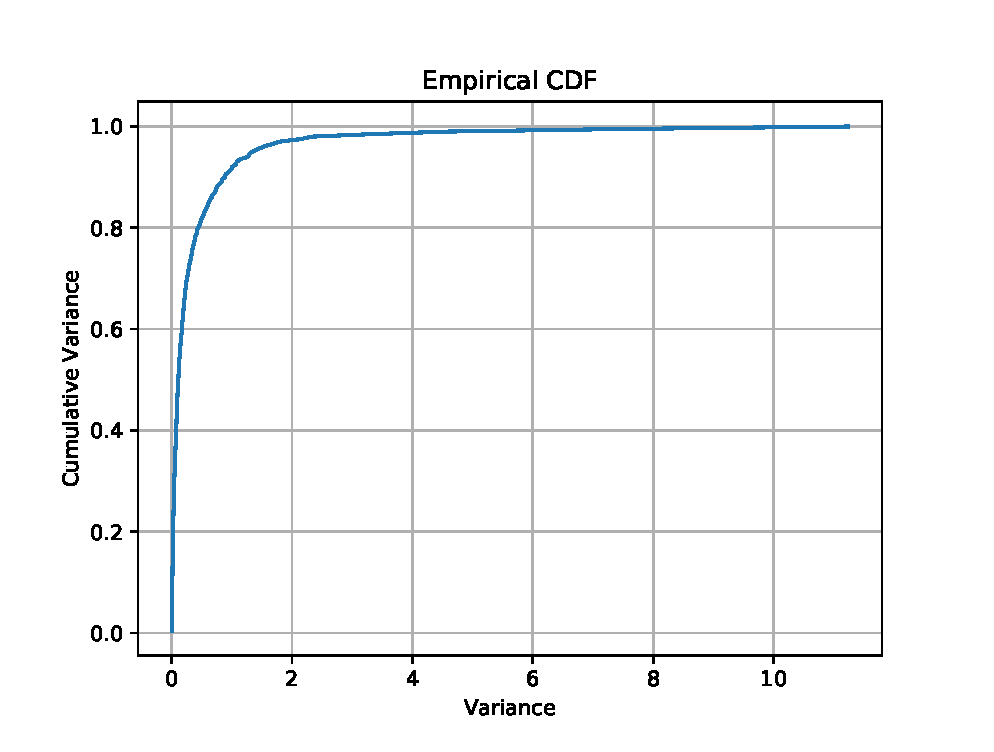
\includegraphics[height=6cm, width=9cm]{figures/pca-svm-rfe_raw_variance_ecdf.eps}
     \caption{Empirical CDF of variance.}
     \label{fig:fig1}
\end{figure}

Depois da extração dos autovalores e percentual da variância explicada, é decidida a quantidade de fatores a serem retirados para análise. Para isso, o Gráfico 1 em que o total de autovalores está no eixo das ordenadas e os autovalores  no eixo das abscissas, auxilia na identificação. Esse gráfico consiste no ranking dos autovalores (eixo x), relacionado com o valor de cada autovalor (eixo y). Verifica-se que uma queda menos acentuada ocorreu entre o quarto e o quinto autovalor e analisando-se os autovalores superiores a 2, observa-se que pode-se considerar até o vigésimo valor já que a partir daí os valores dos autovalores sucessivos são praticamente constantes.
 
Visando encontrar os planos fatoriais realizou-se uma rotação dos eixos, onde as cargas fatoriais mais elevadas são as responsáveis pelas denominações das componentes e são estatisticamente significativas. As rotações de eixos melhor expressam a dispersão de dados. No modelo fatorial final, as variáveis das medidas estão maximizadas e as relações entre dimensões suavizadas (Vicini, 2005).
Para esta análise buscam-se valores que possuem significância maior que 0,7, mostrando que a correlação entre as variáveis está de moderada a forte (Vicini, 2005). Essa identificação não seria possível sem a rotação dos eixos, possibilitando assim a melhor visualização das variáveis mais significativas em cada componente. Tal rotação mantem os eixos perpendiculares entre si, ou seja, ortogonais e a variabilidade do sistema não é alterada, apenas as coordenadas dos eixos são rotacionadas e a inércia do sistema fica inalterada. 
A partir dos valores obtidos pela rotação das componentes principais, podem-se obter valores com significância maior que 0,7. Logo, foi possível a identificação das variáveis significantes de cada componente principal.
Para visualização desses fatores foi utilizado o gráfico de dispersão (Gráfico 2). O Gráfico 2 mostra a caixa de seleção de variáveis e comandos para ACP em que se utilizam os fatores 1 e 2, eixo x e eixo y respectivamente. O objetivo deste gráfico é fazer os planos principais com a nuvem de pontos dos indivíduos, no caso as 349 instituições, destacando o posicionamento das respostas das instituições classificadas pelo iGovTI. Tal gráfico se baseia na rotação dos componentes principais. Para a elaboração do Gráfico 2 apenas os  e  foram utilizados.
 
\begin{figure}[h!]
     \centering 
     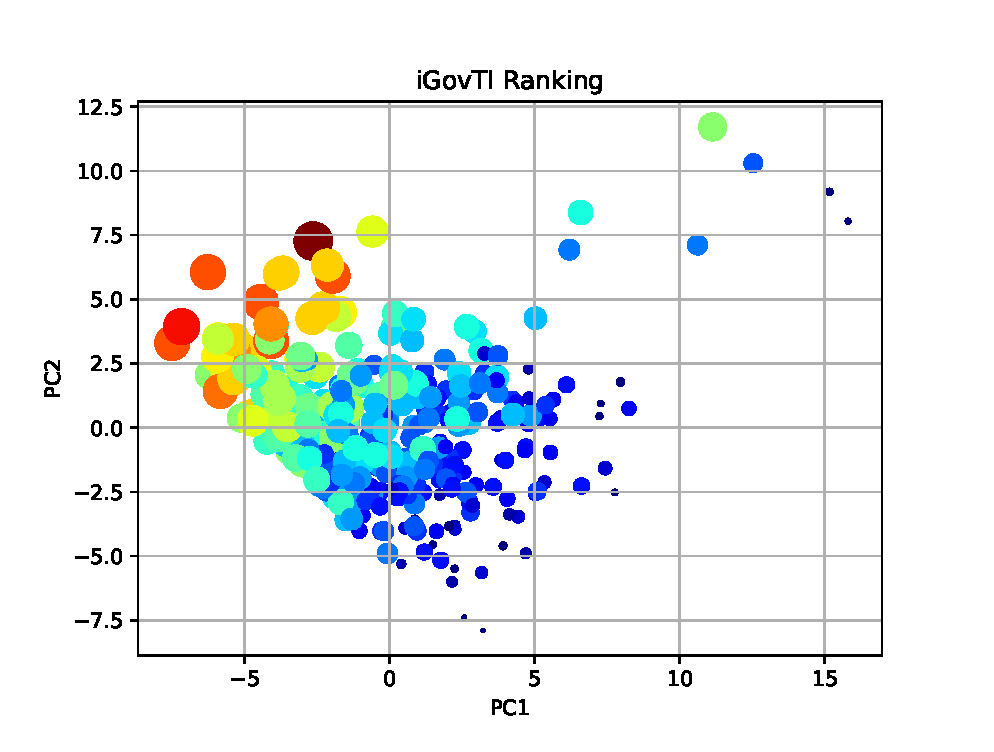
\includegraphics[height=6cm, width=9cm]{figures/pca-svm-rfe_raw_igovti_ranking_pc2.eps}
     \caption{iGovTI ranking from 2 principal components.}
     \label{fig:fig1}
\end{figure}

No Gráfico 2, para analisar apenas a , projetam-se os pontos sobre o eixo da e se tem três grupos (V, II e I). O mesmo processo se aplica a analise da . Assim, observam-se três grupos (V, IV e III). Para cada grupo se seleciona apenas uma variável representativa, o restante é desconsiderado, uma vez que cada grupo significa correlação.
Para o grupo I, tomam-se as variáveis Q16d, Q16e e Q16f que são descorrelacionadas, já no grupo II a questão Q16g é questão selecionada. Ambos os grupos não apresentam FCS. Essas questões denotadas Q16, referem-se a Subdimensão 1.6 (A Alta Administração Utilizou Informações Fornecidas pela Auditoria Interna). Tal subdimensão verifica a participação da auditoria interna das instituições para o preenchimento do questionário. 
% Já no grupo III, que não tem FCS, a variável Q53_Relev é a selecionada; precedidas do grupo IV que também não apresenta FCS. Ressalta-se que ambas as questões apuram a relevância de determinado item. Pela análise ACP, o grupo V mostra as questões que não são representadas pelas  e , é justamente este grupo que contem os FCS.
Depois, buscou-se por meio da análise das ,  e a identificação de FCS (Gráfico 3). O Gráfico 3 mostra a análise dessas componentes principais que revela a existência de três grupos. 

A análise do Gráfico 3 mostra revela a existência de três grupos (VI, VII e VIII). O grupo I contém a variável Q51l que corresponde a FCS e o grupo II também mostra FCS, a variável Q23b.
Na identificação das variáveis significativas das primeiras 20 componentes principais, com os autovalores superiores a 1, as questões que mais contribuem são Q16b (para responder às questões do grupo 2. Estratégias e planos), Q16c (para responder às questões do grupo 3. Informação e conhecimento), Q16d (para responder às questões do grupo 4. Pessoas), Q16e (para responder às questões do grupo 5. Processos) e Q16f (para responder às questões do grupo 6. Resultados da gestão), todas da dimensão “Governança corporativa e de TI, a alta administração utilizou informações fornecidas pela auditoria interna (ou instância equivalente)”. Nota-se que as variáveis Q16, citadas anteriormente, fazem parte do grupo I do Gráfico 2. Ao total foram identificadas 29 variáveis dos 20 primeiras componentes principais (autovalores maiores que 1) das variáveis com significância maior que 0,7. O Quadro 8 mostra quais são essas variáveis significativas. 

No Quadro 8, verificou-se as variáveis que são FCS, de acordo com resultado da pesquisa apresentada na Subseção 4.1. Das 30 questões apenas 5 são FCS, de acordo com classificação obtida por meio de pesquisa qualitativa, quais sejam: Q12c (designou representantes de todas as áreas relevantes para o negócio institucional para compor o Comitê de TI); Q23b (a instituição aprovou e  publicou PDTI interna e externamente); Q51l (gestão de configuração de ativos); Q53e (formalizou a política corporativa de segurança da informação); Q57h (os pagamentos são feitos em função da mensuração objetiva dos resultados entregues e aceitos.
Ainda no Quadro 8, chama-se atenção as ,  e. Nelas constam variáveis com valor positivo ou negativo. Tal fato significa que quanto maior for a resposta de uma questão menor será a da outra. Frisa-se que isto só vale para questões que estejam em uma mesma variável ACP. Caso as questões tenham sinais diferentes (i.e. os elementos dos autovetores), mas em ACP diferentes o sinal positivo e negativo não importa. 
A análise das categorias (Quadro 5) relacionadas às variáveis revela: Q53e referente à Categoria Processos de Gestão de Serviços de TI em Desenho do Serviço que mostrou porcentual igual a 53,85\%; Q57h se liga à Categoria Gestão de Contratos que teve porcentual de 38,46\%; Q23b se vincula à Categoria PDTI que teve 38,46\%. A variável Q51l se relaciona à Categoria Processos de Gestão de Serviços de TI em Transição de Serviços com 19,23\%.
Devido ao baixo percentual de 16,66\% de identificação de FCS do Quadro 8, realizou-se a análise das variáveis que completam as 51 componentes principais, referentes aos 51 autovalores do Quadro 7. Nesta identificação, foram identificadas 33 variáveis, sendo que 8 são FCS, 24,24\% (Quadro 9). Somando os totais obtidos pelo Quadro 8 e pelo se tem, 20,63\% de variáveis que são FCS.

Já o Gráfico 4 mostra a caixa de seleção de variáveis e comandos para ACP em que se utilizam os fatores 1 e 2, eixo x e eixo y respectivamente. O objetivo deste gráfico é fazer os planos principais com a nuvem de pontos dos indivíduos, no caso as 349 instituições.  

O Gráfico 4 representa a relação entre os 2 principais componentes, que representam as questões ou variáveis com maiores autovalores, assim cada ponto representa a relação entre uma instituição e seus 2 principais componentes obtidos por meio de ACP. Cada ponto deste gráfico representa a classificação da instituição em relação a sua classificação no iGovTI de 2012. A partir do resultado apresentado no gráfico 4 é possível identificar um padrão formado pela localização dos componentes principais das organizações com maior índice, onde as organizações com maior iGovTI tiveram valores relativamente semelhantes para seus 2 componentes principais, entretanto ainda não é possível obter uma separação clara entre os resultados. Fazendo-se um corte no eixo das abcissas, a partir do ponto (-8,8, 0), destacam-se 23 instituições à esquerda desse ponto (Quadro 5). 

Dessas instituições, 22, são consideradas pelo TCU como aprimoradas, ou seja, 95,65\%. Apenas a instituição 346 é avaliada como intermediária.
Após a análise ACP, verifica-se que a mesma não é útil para a análise da Hipótese 2. Para responder a essa hipótese, é necessária a execução dos algoritmos de classificação da Subseção 4.4 e da Subseção 4.5.

\subsection{Máquinas de Vetores de Suporte}

Para prever a classificação de uma instituição de acordo com suas respostas para as questões do questionário iGovTI, foram avaliados algoritmos de classificação que pudessem apresentar acurácia para a classificação de organizações de acordo com o iGovTI. Uma vez encontrado um algoritmo capaz desta classificação, é possível utilizar o algoritmo selecionado em conjunto com técnicas de feature selection para identificar as questões mais relevantes para a classificação da instituição de acordo com o iGovTI.
Assim, para a definição do algoritmo de classificação foram realizados testes em 21 algoritmos, a seguir é apresentada uma listagem dos algoritmos avaliados e a taxa de acerto de classificação obtida: 

k-nearest neighbors \cite{fukunaga1975branch}	0.714286
Elastic Net \cite{zou2005regularization}	0.831531
Lasso \cite{tibshirani1996regression}	0.827440
LinearRegression \cite{draper2014applied}	0.360878
LogisticRegression \cite{hosmer2013applied}	0.771429
LDA \cite{martinez2001pca}	0.628571
SVM \cite{hearst1998support}	0.914286
SVM Regression \cite{smola2004tutorial}	0.826885
Linear SVM \cite{fan2008liblinear}	0.714286

O algoritmo que obteve maior sucesso para classificação foi o SVC, que é uma implementação de Máquina de Vetores de Suporte aplicado para a classificação. SVC apresentou uma taxa de acerto de 91,4\%. Para a avaliação dos algoritmos, utilizamos uma metodologia que divide os dados dos questionários pelo iGovTI entre questões que serão utilizadas para aprendizado do algoritmo e questões que serão utilizadas para comparativo de predições. Para treinar o algoritmo utilizou-se 90\% dos dados e os 10\% restantes foram utilizados para avaliar a eficiência de classificação dos algoritmos, comparando a taxa de acerto entre as predições feitas e os valores reais de classificações de organizações pelo iGovTI. 

Uma vez identificado um algoritmo capaz de efetuar a classificação desejada, o próximo passo é identificar as variáveis mais relevantes para esta classificação. Para isso, será utilizado o algoritmo ERV. 

A ERV pode usar vários algoritmos de classificação como critério de seleção das variáveis mais importantes, escolhemos o algoritmo SVC por ele ter apresentado maior acurácia entre os algoritmos de classificação avaliados. Ainda é necessário definir o quantitativo de variáveis mais importantes a serem selecionadas. A partir da pesquisa de identificação por meio de entrevistas na APF, identificou-se 54 variáveis consideradas FCS, este critério foi utilizado para determinar o quantitativo de variáveis mais importantes para a classificação.

Assim, aplicaram-se o algoritmo ERV utilizando o SVC como critério para a seleção das variáveis mais importantes para a classificação, selecionando as 54 variáveis que correspondem aos FCS levantados nas entrevistas com os executivos de TI. Os resultados mostraram que 69,9\% das variáveis foram classificadas da mesma forma que os FCS identificados anteriormente (Quadro 10) por meio de pesquisa qualitativa.

\section{Conclusion}
\label{sec:conclusion}

pca make possible visual discriminative analysis of reduced dataset but it is not easy make correlation betwee extracted features and its original, therefore it is necessary adictional techniques to identify CSF.

SVM have been shown to generalize well even for small sample classification[8]. SVM presents high performance to reproduce the iGovTI classification and can be used for RFE in order to identify CSF

The selected features revealed by RFE are quite similar to the qualitative analysis of Ramos \emph{et al} \cite{ramos2016information}.